% !Mode:: "TeX:UTF-8"
\section{研究方案及进度安排}

\subsection{服务不确定性事件及服务状态模型}

\subsubsection{服务方案}

使用服务流程表示当前执行中的服务方案,表示为如式(\ref{splan})所示。
\begin{equation}\label{splan}
SPlan = \left( {A,E,fc,dc} \right)
\end{equation}
\begin{tabularx}{\textwidth}{@{}l@{\quad}l@{\pozhehao }X@{}}
    式中
    & ${A}$ & 活动集合,表示为~$\{{a_1}, {a_2},...,{a_n}\}$ ~; \\
    & ${E}$ & 活动之间的时序依赖关系,表示为~$\{{e_1}, {e_2},...,{e_n}\}$ ~;\\
    & ${fc}$ & 服务若执行失败,提供方需要支付给客户的补偿金;\\
    & ${dc}$ & 表示服务若执行延期,每单位时间延迟需要支付给客户的补偿金。
\end{tabularx}\vspace{\wordsep}

针对每个活动,可表示为如如式(\ref{a})所示。
\begin{equation}\label{a}
{a_i} = ({CS_i}, {S_{i0}}, {LST_i}, {LET_i})
\end{equation}
\begin{tabularx}{\textwidth}{@{}l@{\quad}l@{\pozhehao }X@{}}
    式中
    & ${CS_i}$ & 活动的可替换服务集;\\
    & ${S_{i0}}$ & 当前被选中用于执行该活动$i$的具体服务;\\
    & ${LST_i}$ & 最晚开始时间;\\
    & ${LET_i}$ & 最晚结束时间;
\end{tabularx}\vspace{\wordsep}

针对活动之间的依赖关系,一般的服务流程中存在各种复杂结构关系\citeup{jaeger2004qos},本文考虑串行与并行两种关系,并使用如式(\ref{e})表示,其意义是活动${a_j}$需要在活动${a_i}$执行完成后才能开始执行,在~DAG~图中体现的则是从结点${a_i}$到结点${a_j}$之间有一条有向边。
\begin{equation}\label{e}
e = ({a_i},{a_j})
\end{equation}

\subsubsection{不确定性事件}

本课题关注的是服务执行过程中从外界可观测到的事件,即站在服务使用者的角度观察系统的运行状态,而不关心服务执行环境内部是何种原因而产生的事件。这样做的原因是服务方案通常是由服务中介方负责构建的,方案中使用的各服务并不受其控制,故只能从外部观察。

事件可表示为如式(\ref{event})所示,其中t为事件发生的时刻,a为事件所涉及的活动,EType表示事件的类型。
\begin{equation}\label{event}
event = (t, a, EType)
\end{equation}
\begin{tabularx}{\textwidth}{@{}l@{\quad}l@{\pozhehao }X@{}}
    式中
    & $t$ & 事件发生的时刻;\\
    & $a$ & 事件所涉及的活动;\\
    & $Type$ &事件的类型。
\end{tabularx}\vspace{\wordsep}

考虑事件的类型~$EType$~。服务执行过程中的产生的事件分为两大类:正常事件、不确定性事件。前者是一项活动按计划正常开始和正常执行结束时所发出,后者是指活动未按预期开始或结束,或者执行失败。按照事件触发的机制,可分为以下三类:

\begin{itemize}
\item 由定时器所触发的事件,表示某活动未在期望时间点上开始执行或执行完成。服务执行引擎根据服务方案中为每个活动预设的最晚开始和最晚结束时刻对服务执行进行监控,如果到达~$LST_i$~或~$LET_i$~时刻活动未能开始或结束,将发出以下两类事件:

$E_{01}$:~活动~$a_i$~在当前时刻~$t$~未开始执行,满足~$t>LST_i+\delta$~ (~$\delta$~是一个足够小的时间间隔),一旦系统在~$LST_i+\delta$~时刻未发现~$a_i$~开始执行,则发出该类事件;

$E_{02}$:~与之类似,活动~$a_i$~在当前时刻~$t$~未按计划执行结束,满足~$t>LETi+\delta$~;

\item 由活动的开始执行所触发的事件~($E_{11}$)~。一旦服务活动开始执行,系统即产生该类事件。~$t\le LST_i$~表示活动提前或准时开始,而~$t>LST_i$~表示活动开始迟于计划。

\item 由活动执行结束所触发的事件,可分为以下两种情况:

$E_{21}$:~活动执行失败或错误,未得到期望结果;

$E_{22}$:~活动执行成功。~$t\le LET_i$~表示活动提前或准时执行结束,而~$t>LETi$~表示活动有延迟。

\end{itemize}


\subsubsection{服务执行的状态}

服务流程在执行过程中产生各种正常或不确定事件,导致服务执行不确定状态。本节给出服务执行状态的刻画。

(1)~单个服务的状态

首先定义活动的状态。对某活动~$a_i$~,其状态可表示为~$state(a_i)=STATE\_TYPE^{N/U}<T, C>$~,或简写为~$STATE\_TYPE^{N/U}$~。~$STATE\_TYPE$~可为以下6种类型之一,~$T$~和~$C$~表示~$a_i$~处于当前状态时相比于预期服务方案的时间延迟~(TimeDelay)~和成本溢出~(CostOverflow)~,~$N$~和~$U$~分别表示该状态为正常状态~(Normal)~或不正常状态~(Uncertain)~,正常状态表示时间和成本未超出初始服务方案中对~$a_i$~的时间与成本的规划~$(T\le 0, C\le 0)$~,不正常状态是指当前存在时间延迟或者成本溢出~$(T>0, C>0)$~。对~$NOT\_READY$~、~$FAIL$~、~$CANCEL$~三类状态来说,不存在正常或不正常的分类,可不需标注上标~$N$~或~$U$~。

\begin{itemize}

\item ~($NOT\_READY$):~$a_i$~至少有一个前序活动尚未执行结束,故~$a_i$~尚无开始执行的条件,即~$\exists a' \in \{ {a_j}|\exists e = ( {{a_j},{a_i}} )\} ,state ( {a'} ) \ne FINISH \Rightarrow state ( {{a_i}} ) = NOT\_READY$~。这是所有活动的缺省状态。

\item 待执行($READY$):~若~$a_i$~的所有前序活动均已执行完毕(处于~$FINISH$~状态),且对这些活动的决策动作均非“终止”时,ai具备了执行的先决条件,进入该状态,即~$\forall a' \in \{ {a_j}|\exists e = ( {{a_j},{a_i}} )\} ,state ( {a'} ) = FINISH \wedge Action(a') \ne STOP \Rightarrow state ( {{a_i}} ) = READY$~。当~$a_i$~处于READY状态且产生~$E_{01}$~时,它仍然处于~$READY$~状态;

\item 执行中($EXEC$):~当本活动产生~$E_{11}$~、~$E_{02}$~事件时,~$a_i$~正在执行中,但尚未结束;

\item 执行后失败($FAIL$):~本活动产生~$E_{21}$~事件,~$a_i$~执行结束,但未得到期望输出,执行失败;

\item 执行后成功~($FINISH$):~本活动产生~$E_{22}$~事件,~$a_i$~执行结束,已得到期望结果;

\item 取消~($CANCEL$):~当某活动处于~$READYU$~、~$FINISHU$~或~$FAIL$~状态,并且决策动作将该活动终止时,~$a_i$~被人为取消,服务方案停止执行而完全失败。
\end{itemize}

事件或决策动作导致活动的状态变化,状态之间的转换关系如图~\ref{state_trans}~所示。
\begin{figure}[htbp]
    \centering
    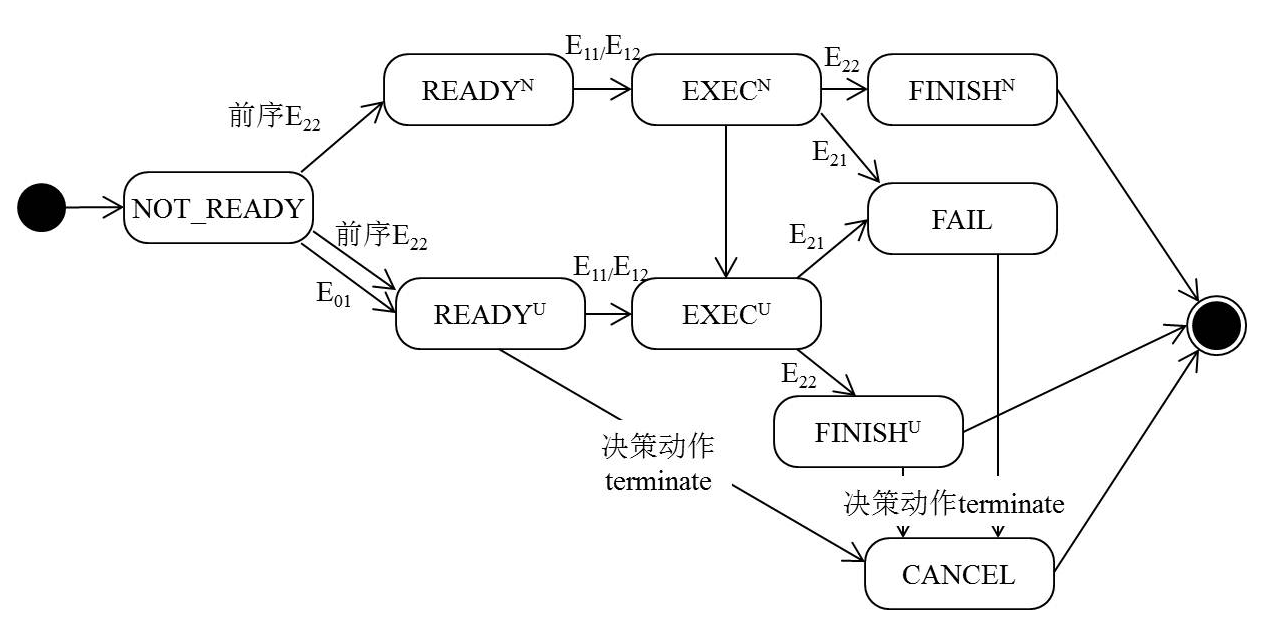
\includegraphics[width = 0.6\textwidth]{state_trans}
    \caption{服务活动的状态转换关系}\label{state_trans}
    \vspace{-1em}
\end{figure}

(2)~服务执行的整体状态

将服务执行“前锋线”~(forward line)~上的各服务活动的状态联合起来,共同表示服务执行的整体状态~state(SPlan)~。
所谓的“前锋线”~(Front Line)~,是指将已经执行的部分和尚未执行的部分分开的一条线,表示为~$FL(SPlan)=\{(a_i, state(a_i))\}$~,它由一组活动及其状态构成,~$prodecessor(FL)$~、~$successor(FL)$~分别为其左侧和右侧的活动集合。处于~$FL$~中的每一个服务,可能是~$READY^{N/U}$~、~$EXEC^{N/U}$~、~$FAIL$~、~$FINISH^{N/U}$~的某一状态,其所有前序活动的状态必须是~$FINISH^{N/U}$~,其所有后序活动的状态必须是~$NOT_READY$~,即
$\forall {a_i} \in FL,state({a_i}) \in \{ READ{Y^{N/U}},{\rm{ }}EXE{C^{N/U}},{\rm{ }}FAIL,{\rm{ }}FINIS{H^{N/U}}\} ;\forall a' \in predecessor(FL),state(a') = FINIS{H^{N/U}};\forall a' \in successor(FL),state(a') = NOT\_READY.$

例如,在某一时刻服务执行状态如图~\ref{front_line}~所示,虚线表示流程执行的前锋线,它左侧的活动~$(a_1, a_2, a_5)$~均处于~$FINISH$~状态,它右侧的活动~$(a_7, a_8, a_9)$~均处于~$NOT\_READY$~状态,而在线上的三个活动~$(a_3, a_4, a_6)$~,分别处于~$READY$~、~$EXEC$~、~$FAIL$~状态。

\begin{figure}[htbp]
    \centering
    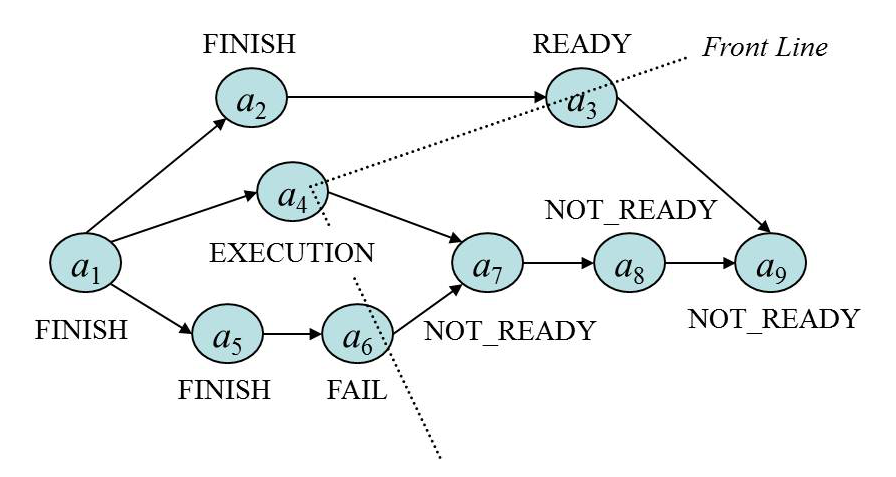
\includegraphics[width = 0.5\textwidth]{front_line}
    \caption{服务方案执行中的状态划分与前锋线}\label{front_line}
    \vspace{-1em}
\end{figure}

~$state(SPlan)$~可分为几类:
\begin{itemize}
\item 执行前: ~$predecessor(FL) = \emptyset ,$ 对 $ \forall {a_i} \in FL,state({a_i}) = READ{Y^N}$~;
\item 执行中: ~$FL \ne \emptyset ,predecessor(FL) \ne \emptyset ,successor(FL) \ne \emptyset $~;
\item 执行结束(成功): ~$FL = \emptyset ,successor(FL) = \emptyset ,$ 对 $\forall {a_i} \in predecessor(FL),state({a_i}) = FINIS{H^{N/U}}$~;
\item 执行结束(失败): ~$FL \ne \emptyset ,$ 且 $\exists {a_i} \in FL,state({a_i}) = FAIL$~;
\end{itemize}

面向不确定性的优化决策的目标可表述为:以最小的时间延迟和成本溢出,使服务可最大概率的进入到“成功结束”状态。

\subsection{软件层面面向不确定性的服务自适应决策模型}

\subsubsection{决策动作}

针对每一种不确定性,有多种可用的决策动作,需要识别出可能的决策动作,对其分类,并估算“若采取某项决策动作,可能会付出的直接/间接成本,以及对服务预期收益的影响”。将每一次决策表示为四元组~$SPlan,{a_i},state,action,SPlan'$~,含义是:当前服务执行方案~$SPlan$~,出现了不确定性事件导致某服务活动~$a_j$~进入状态~$state_j$~,此时采取对策~$action$~,得到新的方案~$SPlan'$~。

本文将决策动作归纳为五类:
\begin{enumerate}
\item 终止~(terminate):~停止活动的执行,~$state(a_i)=FAIL$~,客户需求无法满足,服务失败,~$SPlan'=\emptyset $~;
\item 不作为~(continue):~不做额外的调整对策,继续按原方案执行下去,~$SPlan'=SPlan$~;
\item 重试~(retry):~重新执行出现异常的活动,即令~$state(a_i)=EXECU(T, C)$~;
\item 替换~(substitute):~为出现异常的活动~$a_i$~从其候选服务集~$CS_i$~中选择一个新服务~$S_{ij}$~替换原服务~$S_{i0}$~,并重新启动执行~$a_i$~,即:~${S_i}_0 \leftarrow {S_{ik}}$~,其中~${S_{ik}} \in C{S_i}$~;
\item 重组~(recompose):~对当前前锋线的右侧尚未执行的服务活动进行重组,形成替代方案并启动执行。这相当于对多个服务要素进行替换操作。即:将多个服务~${S_i}_0,{S_{i + 1,0}}, \ldots ,{S_j}_0$~分别替换为~${S_i}_k,{S_{i + 1,k}}, \ldots ,{S_j}_k$~, 其中~${S_i}_k \in C{S_i},{S_{i + 1,k}} \in C{S_{i + 1}}, \ldots ,{S_j}_k \in C{S_j}$~。
\end{enumerate}

终止、不作为和重试对服务方案的结构无影响,替换相当于为某一活动进行服务选择,重组相当于对后续未执行服务流程进行服务重组。替换和重组是为尚未执行的一个或多个活动选择时间更短或价格更低的候选服务,以此来消除之前因为不确定事件所导致的时间延误或成本溢出,替换可相当于对1个活动进行重新选择和组合服务,而在工作流不变的情况下的重组相当于对多个活动进行替换和组合服务。在此之前,需要根据~$SPlan$~的当前状态动态生成替换和重组的目标函数,使得当前造成的时间延误和成本溢出将最大程度的降低。

\subsubsection{事件、决策和状态之间的关系}

在服务方案执行过程中,某时刻若产生某一不确定性事件,则会导致某一活动状态发生变化(若是正常事件,也可能不发生变化)。此时进行决策,根据决策动作修正服务方案并更新受影响的活动状态,继续投入执行。如此循环往复,直到服务停止或者执行成功。对活动执行前、执行后的状态,一旦该状态产生,马上进行决策;对活动执行中的状态,等活动达到执行后的某一状态时再进行决策。

需要说明的是,虽然决策针对服务的整体状态,但是每次动作只针对前锋线上的某一个活动进行。若前锋线上多个活动均处于异常状态,那么多个导致异常状态的事件必然是有先后次序到达的,因而决策也会随事件到达的先后次序进行。因此,决策只需要针对单一活动的状态进行,不需要针对多个异常活动进行。

针对服务所处的不同状态,可能采取的决策动作是上述五类中的子集。表~\ref{state_action}~的前四列给出了某一活动处于不同状态时可能采用的决策动作集合,以及决策之后可能导致的新状态。

\begin{table}[htbp]
    \caption{服务状态与决策动作之间的关系}
    \vspace{-0.5em}\label{state_action}\centering\zihao{5}
%    \includegraphics[width = 0.9\textwidth, bb=0 0 800 600]{state_action}
    \includegraphics[width = 0.9\textwidth]{state_action}
\end{table}

\subsubsection{决策收益}
各种动作的目标是“使不确定性造成的损失尽可能小”,但并不保证服务一定能够从异常状态完全回到正常轨道,因此需要分析每种决策对服务执行的影响,计算其损失/受益,以此作为优化决策的依据。

决策动作对原有的服务方案进行了调整,对它的收益度量从以下三个因素入手:

(1)~使服务可以继续向后执行的概率。一般情况下服务失败后需支付给顾客的补偿~$(fc)$~较高,因此决策动作应尽可能保证服务可以继续执行下去。除了补偿上的考虑之外,还考虑到服务执行失败可能造成的客户流失。设决策动作之后,受影响的活动(可能为当前活动,也可能为下一步活动)执行成功的概率为r,那么该部分代价是~$(1-r) \times fc$~。

(2)~若造成时间延迟而需支付的延误成本。设延误时间为~$\Delta T$~,那么该部分的代价是~$\Delta T \times dc$~。

(3)~所引入的新成本~$\Delta C$。~对终止和不作为两种动作来说,新成本为0;对重试动作来说,新成本为重新支付的当前服务使用价格;对替换动作来说,新成本为所选新替代服务的使用价格;对重组动作来说,新成本为所选的多个替代服务的使用价格与原方案中相应服务的使用价格之差。
因此,在当前状态下state采取决策动作action所带来的总收益是:
~$Reward =  - ((1 - r) \times fc + \Delta T \times dc + \Delta C)$~,其中~$r$~、~$\Delta T$~、 ~$\Delta C$~的计算方式如表~\ref{state_action}~右侧的三列所示。

\subsubsection{不确定性触发关系图~(UTG)~}
不确定性本身蕴含着服务的一种状态(不正常状态),它是可以传播的,若不采取任何对策(不作为),任由某一不确定性蔓延下去,将会造成更严重的后果(成本溢出、时间延误、执行失败)。即使采取了某一种对策,弥补了某些潜在后果,但可能不会完全弥补,因此也会扩散。这里提出不确定性触发关系图~(Uncertainty Triggering Graph, UTG)~表达~UC~之间的触发关系。利用~UTG~来计算不确定性事件及决策动作所引发的直接和间接代价。

UTG可表示为包含两类节点和两类边的有向图~UTG = ~$(rs, SS, AS, TSA, TAS)$,其中:
\begin{itemize}
\item ~$rs=(a_i, state_i)$~表示根状态,代表活动~$a_i$~处于~$state_i$~时所生成的UTG;
\item ~$SS={ss}$~为状态节点集合,其中包含两类节点:第一类为原子状态~$ss=(a_j, state_j)$~,第二类为嵌套的~UTG~根结点,可扩展为一棵完整的~UTG~树;
\item ~$AS={action}$~为决策动作节点的集合;
\item ~$TSA=ss \to action$~表示状态节点到决策动作节点的有向边;
\item ~$TAS=action \to ss$~表示决策动作节点到状态节点的有向边,它具有三个属性:~$tp$~(该状态转移的概率)、~$\Delta T$~(该状态转移所造成的时间延迟)、~$\Delta C$~(该状态转移所造成的成本增加)。
\end{itemize}

如图~\ref{utg_tree}~给出了UTG示意图,其中菱形框表示根状态,圆形节点表示原子状态,矩形框表示决策动作节点,箭头表示~$TSA$~和~$TAS$~。

\begin{figure}[htbp]
    \centering
    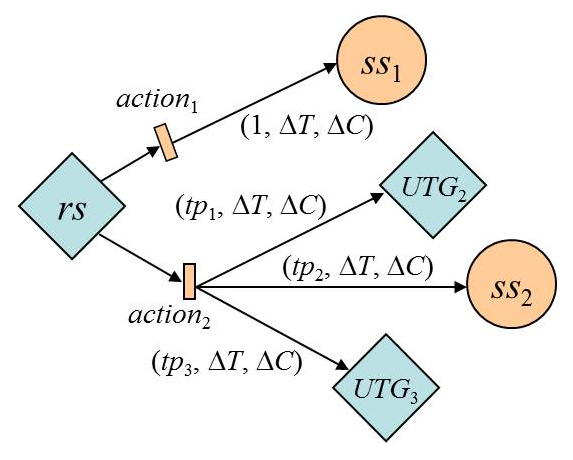
\includegraphics[width = 0.3\textwidth]{utg_tree}
    \caption{不确定性事件触发关系图~(UTG)~}\label{utg_tree}
    \vspace{-1em}
\end{figure}

在~UTG~模型中,状态节点可以是一棵~UTG~的根节点,这代表了不同~UTG~之间的连接(不同活动的不确定性状态之间的转换)。若将此类~UTG~节点展开,即可形成如图~\ref{many_utg_tree}~所示的形态。

\begin{figure}[htbp]
    \centering
    \includegraphics[width = 0.5\textwidth]{many_utg_tree}
    \caption{多棵UTG的连接~(UTG)~}\label{many_utg_tree}
    \vspace{-1em}
\end{figure}

如图~\ref{utg_example}~给出一个小例子。假设服务方案是由三个活动~$(a_1, a_2, a_3)$~串行构成的流程,图~(a)~表示活动~$a_1$~在~$READY^U$~状态下的~UTG~,~(b)~表示活动~$a_1$~在~$FINISH^U$~状态下的~UTG~,~(c)~表示~$a_1$~在~$FAIL$~状态下的~UTG~。

\begin{figure}[htbp]
    \centering
    \includegraphics[width = 0.5\textwidth]{utg_example}
    \caption{~UTG~的三个例子}\label{utg_example}
    \vspace{-1em}
\end{figure}

~UTG~的结构与服务方案的流程结构密切相关。当出现不确定性事件之后,更新相关活动、状态和前锋线的信息,进而根据表~\ref{state_action}~的相关信息生成~UTG~。

\subsection{业务层面面向不确定性的服务自适应决策模型}




\subsection{基于MDP的不确定性决策方法}
马尔科夫决策过程~(MDP)\citeup{liuke2004}~将马尔可夫过程与确定性的动态规划相结合,决策者周期或连续观察随机动态系统,序贯的做出决策,系统下一步的状态是随机的,并且其状态转移概率具有马尔可夫性。决策者根据新观察到的状态,再作新的决策,依此反复地进行。通过此种决策,使系统运行的全过程达到某种最优运行效果,选取控制系统发展的最优策略。

\subsubsection{模型}

服务执行过程中面临的各种不确定性以及对其所做出的决策,符合~Markov~决策过程的定义。因此,采用基于~MDP~的方法进行服务自适应演化过程中的决策,根据当前服务执行状态、发生的不确定性事件、不确定性事件之间的触发关系~(UTG)~,考虑未来的收益和代价,做出当前不确定状态下的最优决策。

按照~MDP~的数学模型,需要首先建立决策时刻~$T$~、服务状态~$S$~、决策动作~$A$~、转移概率~$P$~、代价~$Reward$~的数学表达。

(1)~时刻~$T$~: 前服务环节执行中/执行后发生不确定事件、或者预知到尚未执行的环节将会发生不确定事件时开始决策,此时为时刻0。如图4所示的多棵~UTG~连接形成完全触发关系图,叶子结点的状态处于最终时刻~$V$~,“完全触发关系图”的层数是周期个数。这是一个不定周期的时刻序列。

(2)~状态~$S$~: 服务前锋线上的所有活动的状态即可表示为服务流程的状态,原因是前锋线上的活动状态已知,则可知所有活动的状态。将服务流程的所有活动的六种状态组成一个状态集合,形成~MDP~状态~$state$~, 即~$state =  < state({a_1}),state({a_2}), \ldots ,state({a_n}) >$~,每个状态附着两个参数(~$T$~和~$C$~);

(3)~动作~$A$~:共有终止、不作为、重试、替换、重组五个动作,不同状态下可执行的动作集合有所不同(见表~\ref{state_action}~)。

(4)~转移概率~$P$~:转移概率由当前的决策动作和服务活动的状态联合决定,即~$p(state_j|state_i,action)$~的值有以下几类情况:
\begin{itemize}
\item ~$1;~if~action = continue/terminate$~
\item ~$reliability;~if~action = retry/substitute/re-compose~ \& ~ state_j = FINIS{H^{N/U}}$~
\item ~$1 - reliability;~if~action = retry/substitute/re-compose ~\& ~ state_j = FAIL$~
\end{itemize}
其中~$reliability$~指的是将要执行的服务端可靠性,若有多个服务,则是多个服务可靠性之积。

(5)~报酬函数~$Reward$~:在4.2.3节中给出。

\subsubsection{算法}

基于上述五个方面的基本定义,采用有限阶段向后递归迭代~MDP~算法进行最优决策序列的求解,得到对当前服务的决策动作。

算法:基于~MDP~的服务不确定性优化决策

输入:服务方案~$SPlan$~、与当前发生的不确定性事件相关的活动~$activity$~、
~$SPlan$~中各个活动的当前状态;

输出:最优马氏策略及其成本

步骤1~根据出现故障的活动~$a$~,按照表~\ref{state_action}~构造~UTG~,并将多棵~UTG~连接形成“完全触发关系图”,从而形成状态转移表;

步骤2~定义当前的不确定状态为时刻0,以此生成向后衍生的UTG,直至服务方案最后一个结点,此时为最终时刻V。从而生成0到~$V$~的~$V+1$~个时刻的若干个状态、若干个动作、相应的转移概率报酬;

步骤3~令~$t=V$~,且对所有~$V$~时刻的状态~$state_V \in S$~,令~${u_V}( {state_V} ) = Reward_V( {state_V} )$;

步骤4~如果~$t=0$~,则~$\pi  = (f_0,f_1,\ldots ,f_{V-1})$~为最优的马氏策略,而~${u_0}( state_0)$~为最优的值函数,算法停止。否则,令~$t=t–1$~,进入步骤5;

步骤5~对所有~$state_t \in S$~,计算

\begin{equation}\label{backward_mdp}
\begin{array}{l}
{u_t}(stat{e_t}) = \mathop {\max }\limits_{action \in Action(stat{e_t})} \{ Rewar{d_t}(stat{e_t},action)\\
{\rm{                        }} + \sum\limits_{stat{e_{t + 1}} \in S} {{p_t}(stat{e_{t + 1}}|stat{e_t},action){u_{t + 1}}(stat{e_{t + 1}})} \} 
\end{array}
\end{equation}

并记集合

\begin{equation}\label{backward_mdp_arg}
\begin{array}{l}
Actio{n_t}(stat{e_t}) = \mathop {\arg \max }\limits_{action \in Action(stat{e_t})} \{ Rewar{d_t}(stat{e_t},action)\\
{\rm{                       }} + \sum\limits_{stat{e_{t + 1}} \in S} {{p_t}(stat{e_{t + 1}}|stat{e_t},action){u_{t + 1}}(stat{e_{t + 1}})} \} 
\end{array}
\end{equation}

任意取~$f_t(state_t) \in Action_t(state_t)$~,于是定义了~$t$~时刻的决策规则~$f_t$~。而0时刻的决策~$f_0$~则是对当前故障时刻的故障状态采取最优的直接动作。

步骤6~返回步骤3。

\subsection{原型系统}
文本

\subsection{海运物流业务的不确定性决策系统}
文本


\subsection{预期达到的目标和取得的研究成果}
文本

\subsection{进度安排}
文本
